%\subsection{32-25-12-HaNoi-Amsterdam-L2}
\caulc
\Opensolutionfile{ans}[ans/ans-32-25-12-HaNoi-Amsterdam-L2-LC]
\begin{ex}%[Đề khảo sát TN THPT 2025 môn Toán lần 2 trường chuyên Hà Nội – Amsterdam] %[Anh Lan Dương, 32-25-12-HaNoi-Amsterdam-L2]%[2D4N1-1]
	Cho hàm số $f(x) = e^x - \sin x$. Khẳng định nào dưới đây là đúng?
	\choice
	{\True $\displaystyle\int f(x) \, \mathrm{d}x = e^x + \cos x + C$}
	{$\displaystyle\int f(x) \, \mathrm{d}x = e^x - \cos x + C$}
	{$\displaystyle\int f(x) \, \mathrm{d}x = e^x - \sin x + C$}
	{$\displaystyle\int f(x) \, \mathrm{d}x = e^x + \sin x + C$}
	\loigiai{Theo công thức tính nguyên hàm, ta có:
	$\displaystyle\int f(x) \, \mathrm{d}x =
	\displaystyle\int (e^x - \sin x) \, \mathrm{d}x =
	e^x + \cos x + C$.}
\end{ex}

\begin{ex}%[Đề khảo sát TN THPT 2025 môn Toán lần 2 trường chuyên Hà Nội – Amsterdam] %[Anh Lan Dương, 32-25-12-HaNoi-Amsterdam-L2]%[2D1N1-1]
	Hàm số nào sau đây đồng biến trên $\mathbb{R}$?
	\choice
	{$y = x^3 + 3x$}
	{$y = x^3 - 3x$}
	{$y = \dfrac{x-1}{x+1}$}
	{$y = x^4 - 3x^2 + 1$}
	\loigiai{Ta có: $(x^3+3x)'=3x^2+3> 0, \forall x\in\mathbb{R}$. Nên $y = x^3 + 3x$ đồng biến trên $\mathbb{R}$.}
\end{ex}

\begin{ex}%[Đề khảo sát TN THPT 2025 môn Toán lần 2 trường chuyên Hà Nội – Amsterdam] %[Anh Lan Dương, 32-25-12-HaNoi-Amsterdam-L2]%[2D3H1-3]
	Cho mẫu số liệu ghép nhóm về khoảng tuổi và số người như bảng sau:
	\begin{center}
		\begin{tabular}{|c|c|c|c|c|c|c|}
			\hline
			Khoảng tuổi & $[22; 31)$ & $[31; 40)$ & $[40; 49)$ & $[49; 58)$ & $[58; 67)$ & $[67; 76)$ \\
			\hline
			Số người & $33$ & $23$ & $23$ & $16$ & $16$ & $9$ \\
			\hline
		\end{tabular}
	\end{center}
	Khoảng tứ phân vị (làm tròn kết quả đến hàng phần trăm) của mẫu số liệu ghép nhóm đã cho bằng
	\choice
	{$13,62$}
	{\True $25,01$}
	{$11,38$}
	{$32,18$}
	\loigiai{ Ta có: $n=120$.
	Tứ phân vị thứ nhất của mẫu số liệu nằm ở vị trí $\dfrac{120}{4}=30$.
	Mà vị trí thứ $30$ nằm ở nhóm $[22;31)$ (nhóm thứ $1$) nên $Q_1\in [22;31)$. Khi đó,
	$$Q_1=a_1+\dfrac{\dfrac{n}{4}-(m_0)}{m_1}\cdot h
	=22+\dfrac{30-0}{33}\cdot 9
	= \dfrac{332}{11} .$$
	Tứ phân vị thứ ba của mẫu số liệu nằm ở vị trí $\dfrac{3\cdot 120}{4}=90$.
	Mà vị trí thứ $90$ nằm ở nhóm $[49;58)$ (nhóm thứ $4$) nên $Q_3\in [49;58)$. Khi đó,
	$$Q_3=a_4+\dfrac{\dfrac{3n}{4}-(m_1+m_2+m_3)}{m_4}\cdot h
	=49+\dfrac{90-(33+23+23)}{16}\cdot 9
	= \dfrac{883}{16} .$$
	Khi đó, $\Delta Q=Q_3-Q_1=\dfrac{4401}{176} \approx 25,01.$
	}
\end{ex}

\begin{ex}%[Đề khảo sát TN THPT 2025 môn Toán lần 2 trường chuyên Hà Nội – Amsterdam] %[Anh Lan Dương, 32-25-12-HaNoi-Amsterdam-L2]%[2H5N2-3]
	Trong không gian $Oxyz$, cho các điểm $A(1; -2; 3), B(-2; 1; 1), C(0; 2; 3)$. Phương trình đường thẳng $d$ đi qua $A$ và song song với đường thẳng $BC$ là:
	\choice
	{$\begin{cases} x = 2 + t \\ y = 1 - 2t \\ z = 2 + 3t \end{cases}$}
	{$\begin{cases} x = 1 - t \\ y = -2 + 2t \\ z = 3 + 2t \end{cases}$}
	{$\begin{cases} x = -1 + 2t \\ y = 2 + t \\ z = -3 + 2t \end{cases}$}
	{\True $\begin{cases} x = 1 + 2t \\ y = -2 + t \\ z = 3 + 2t \end{cases}$}
		\loigiai{
		Vì $d$ song song với $BC$ nên d có véc-tơ chỉ phương là
		$\overrightarrow{u_d}=\overrightarrow{BC}=(2;1;2)$.\\
		Lại có $d$ đi qua A nên ta có phương trình đường thẳng $d$ là
		$\begin{cases} x = 1 + 2t \\ y = -2 + t \\ z = 3 + 2t \end{cases}$
	.}
\end{ex}

\begin{ex}%[Đề khảo sát TN THPT 2025 môn Toán lần 2 trường chuyên Hà Nội – Amsterdam] %[Anh Lan Dương, 32-25-12-HaNoi-Amsterdam-L2]%[1D6N4-2]
	Nghiệm của phương trình $5^{x-1} - 17 = 0$ là:
	\choice
	{\True $1 + \log_5 17$}
	{$1 - \log_5 17$}
	{$-1 + \log_5 17$}
	{$1 + \log_{17} 5$}
		\loigiai{
		$5^{x-1} - 17 = 0
		\Leftrightarrow 5^{x-1} =17 
		\Leftrightarrow x-1 = \log_5 17
		\Leftrightarrow x = 1+ \log_5 17.
		$
	}
\end{ex}

\begin{ex}%[Đề khảo sát TN THPT 2025 môn Toán lần 2 trường chuyên Hà Nội – Amsterdam] %[Anh Lan Dương, 32-25-12-HaNoi-Amsterdam-L2]%[2H5H1-3]
	Trong không gian với hệ trục tọa độ $Oxyz$, mặt phẳng đi qua điểm $A(1; 2; -3)$ và song song với mặt phẳng $(P)\colon x - 2y + z - 4 = 0$ có phương trình là:
	\choice
	{\True $x - 2y + z + 6 = 0$}
	{$x + 2y - 3z + 6 = 0$}
	{$x + 2y - 3z - 6 = 0$}
	{$x - 2y + z - 6 = 0$}
		\loigiai{
		Gọi mặt phẳng cần tìm là $(Q)$.\\
		Vì mặt phẳng $(Q)$ song song với $(P)$ nên $(Q)$ có véc-tơ pháp tuyến là
		$\overrightarrow{n_{(Q)}}=\overrightarrow{n_{(P)}}=(1;-2;1)$.\\
		Lại có $(Q)$ đi qua $A(1; 2; -3)$ nên phương trình mặt phẳng $(Q)$ là 
		$$(x-1)-2(y-2)+(x+3)=0
		\Leftrightarrow x - 2y + z + 6 = 0.$$
	}
\end{ex}

\begin{ex}%[Đề khảo sát TN THPT 2025 môn Toán lần 2 trường chuyên Hà Nội – Amsterdam] %[Anh Lan Dương, 32-25-12-HaNoi-Amsterdam-L2]%[2D1N4-1]
	\immini{
	Hàm số $y = \dfrac{ax+b}{cx+d}$ có đồ thị như hình bên dưới. Đường tiệm cận đứng của đồ thị là đường thẳng có phương trình
	\choice
	{$x = 1$}
	{$x = 2$}
	{$x = -2$}
	{\True $x = -1$}}
	{
			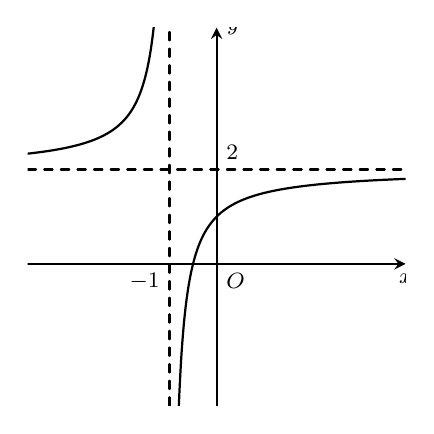
\begin{tikzpicture}[scale=0.6,>=stealth, font=\footnotesize, line join=round, line cap=round]
				\clip (-4,-3) rectangle (4,5);
				% 1. Vẽ các trục tọa độ
				\draw[->, thick] (-4,0) -- (4,0) node[below] {$x$};
				\draw[->, thick] (0,-3) -- (0,5) node[right] {$y$};
				\node[below right] at (0,0) {$O$};
				
				% 2. Vẽ các đường tiệm cận (nét đứt)
				\draw[dashed, thick] (-1,-3) -- (-1,5); % Tiệm cận đứng x = -1
				\draw[dashed, thick] (-4,2) -- (4,2);   % Tiệm cận ngang y = 2
				
				% 3. Điền các giá trị trên trục/tiệm cận
				\node[below left] at (-1,0) {$-1$};
				\node[above right] at (0,2) {$2$};
				
				% 4. Vẽ đồ thị hàm số (y = (2x+1)/(x+1))
				% Nhánh bên trái (x < -1)
				\draw[thick, smooth, samples=100, domain=-4:-1.3] 
				plot (\x, {(2*\x + 1)/(\x + 1)});
				
				% Nhánh bên phải (x > -1)
				\draw[thick, smooth, samples=100, domain=-0.9:4] 
				plot (\x, {(2*\x + 1)/(\x + 1)});
				
			\end{tikzpicture}
}
	\loigiai{
	Quan sát đồ thị hàm số, ta thấy đường tiệm cận đứng của phương trình là $x=-1$.
}
\end{ex}

\begin{ex}%[Đề khảo sát TN THPT 2025 môn Toán lần 2 trường chuyên Hà Nội – Amsterdam] %[Anh Lan Dương, 32-25-12-HaNoi-Amsterdam-L2]%[1H8H5-2]
	Cho hình lập phương $ABCD.A'B'C'D'$ có cạnh bằng $2a$. Khoảng cách từ điểm $A'$ đến đường thẳng $BD$ bằng
	\choice
	{\True $\sqrt{6}a$}
	{$2a$}
	{$\sqrt{5}a$}
	{$2\sqrt{2}a$}
		\loigiai{
	\begin{center}
			\begin{tikzpicture}[line join = round, line cap = round,>=stealth,scale=0.8]
			\path
			(0,0) coordinate (A) 
			(4,0) coordinate (D)
			(-1,-1.5) coordinate (B) 
			($(B)+(D)-(A)$) coordinate (C)
			(0,3) coordinate (A')
			($(B)+(0,3)$) coordinate (B')
			($(C)+(0,3)$) coordinate (C')
			($(D)+(0,3)$) coordinate (D')
			($(B)!0.5!(D)$) coordinate (I)
			;
			\draw[dashed] (A') -- (A) (A) -- (B) (A) -- (D) 
			(A')--(B)	(A')--(D)	(B)--(D)	(A')--(I)
			;
			\draw[] (B) -- (C) -- (D) -- (D') -- (C') -- (B') -- cycle
			(B') -- (B) (C') -- (C) (D') -- (A') -- (B')
			;
			\pic[draw, angle radius=2mm] {right angle=A'--I--B}
			;
			\foreach \p/\pos in {A/left, B/left, C/right, D/right, A'/above, B'/left, C'/right, D'/above,I/below}
			\filldraw[] (\p) circle (1.5pt) node[\pos, black] {\p};
			
		\end{tikzpicture}
	\end{center}
		Vì $A'B,BD,A'D$ là các đường chéo của các mặt hình lập phương nên
		$$A'B = BD = A'D = \sqrt{(2a)^2+(2a)^2}=2a\sqrt{2}.$$
		Hay $\triangle A'BD$ là tam giác đều có cạnh là $2a\sqrt{2}$. \\
		Kẻ $A'I \perp BD$. Khi đó, $d(A',BD)=A'I=A'B\cdot \sin 60^\circ =a\sqrt{6}$.
	}
\end{ex}

\begin{ex}%[Đề khảo sát TN THPT 2025 môn Toán lần 2 trường chuyên Hà Nội – Amsterdam] %[Anh Lan Dương, 32-25-12-HaNoi-Amsterdam-L2]%[2H2N1-3]
	\immini{
	Cho hình lập phương $ABCD.A'B'C'D'$ cạnh bằng $a$. Tính $\vec{AC} \cdot \vec{A'B'}$
	\choice
	{\True $a^2$}
	{$-a^2$}
	{$2a^2$}
	{$-2a^2$}}
		{\begin{tikzpicture}[line join = round, line cap = round,>=stealth,scale=0.8]
			\path
			(0,0) coordinate (A) 
			(4,0) coordinate (D)
			(-1,-1.5) coordinate (B) 
			($(B)+(D)-(A)$) coordinate (C)
			(0,3) coordinate (A')
			($(B)+(0,3)$) coordinate (B')
			($(C)+(0,3)$) coordinate (C')
			($(D)+(0,3)$) coordinate (D')
			;
			\draw[dashed] (A') -- (A) (A) -- (B) (A) -- (D);
			\draw[] (B) -- (C) -- (D) -- (D') -- (C') -- (B') -- cycle
			(B') -- (B) (C') -- (C) (D') -- (A') -- (B')
			;
			\foreach \p/\pos in {A/left, B/left, C/right, D/right, A'/above, B'/left, C'/right, D'/above}
			\filldraw[] (\p) circle (1.5pt) node[\pos, black] {\p};
			
	\end{tikzpicture}}
	\loigiai{
	Áp dụng công thức tính tích vô hướng của 2 véc-tơ, ta có 
	$$\vec{AC} \cdot \vec{A'B'} 
	=\vec{AC} \cdot \vec{AB} = AC\cdot AB \cdot \cos 45^\circ = a \cdot a\sqrt{2} \cdot \dfrac{\sqrt{2}}{2} = a^2.$$
}
\end{ex}

\begin{ex}%[Đề khảo sát TN THPT 2025 môn Toán lần 2 trường chuyên Hà Nội – Amsterdam] %[Anh Lan Dương, 32-25-12-HaNoi-Amsterdam-L2]%[1D2N2-2]
	Cho cấp số cộng $(u_n)$ với $u_1 = 3$ và $u_2 = -6$. Số hạng $u_3$ bằng:
	\choice
	{$12$}
	{$-12$}
	{\True $-15$}
	{$-3$}
		\loigiai{
		Công sai của cấp số cộng là $d=u_2-u_1=-6-3=-9$.\\
		Khi đó, $u_3=u_1+2d=3+2\cdot (-9)=-15$.
	}
\end{ex}

\begin{ex}%[Đề khảo sát TN THPT 2025 môn Toán lần 2 trường chuyên Hà Nội – Amsterdam] %[Anh Lan Dương, 32-25-12-HaNoi-Amsterdam-L2]%[1D6H4-4]
	Bất phương trình $\log_4(x - 5) < 2$ có bao nhiêu nghiệm nguyên?
	\choice
	{\True $15$}
	{$12$}
	{$10$}
	{$8$}
		\loigiai{
		Điều kiện xác định: $x-5>0 \Leftrightarrow x>5$.\\
		Ta có: $\log_4(x - 5) < 2 
		\Leftrightarrow x-5 < 4^2 \Leftrightarrow x<21
		$.\\
		Kết hợp điều kiện xác định, ta có: $5<x<21$. Khi đó, số nghiệm nguyên của phương trình là
		$x\in\{6;7;8;\cdots;20 \}$.
	}
\end{ex}

\begin{ex}%[Đề khảo sát TN THPT 2025 môn Toán lần 2 trường chuyên Hà Nội – Amsterdam] %[Anh Lan Dương, 32-25-12-HaNoi-Amsterdam-L2]%[2D1N2-2]
	Cho hàm số $f(x)$ có bảng xét dấu của $f'(x)$ như sau:
\begin{center}
	
\begin{tikzpicture}
	% Khởi tạo bảng: lgt là độ rộng cột tiêu đề, espcl là khoảng cách giữa các cột x
	\tkzTabInit[lgt=1.5, espcl=2.5]
	{$x$ /1., $f'(x)$ /1.}
	{$-\infty$, $-2$, $0$, $2$, $+\infty$}
	\tkzTabLine{ , +, 0, -, 0, +, 0, +, }
\end{tikzpicture}
\end{center}
	Số điểm cực trị của hàm số đã cho là
	\choice
	{$1$}
	{\True $2$}
	{$0$}
	{$3$}
		\loigiai{
		Quan sát bảng biến thiên, ta thấy $f'(x)$ đổi dấu 2 lần nên hàm số có $2$ cực trị.
	}
\end{ex}
\Closesolutionfile{ans}
%\indapan{6}{ans/ans-32-25-12-HaNoi-Amsterdam-L2-LC}

\cauds
\Opensolutionfile{ans}[ans/ans-32-25-12-HaNoi-Amsterdam-L2-DS]
\begin{ex}%[Đề khảo sát TN THPT 2025 môn Toán lần 2 trường chuyên Hà Nội – Amsterdam] %[Anh Lan Dương, 32-25-12-HaNoi-Amsterdam-L2]%[2D1H4-1]
	Cho hàm số $y = \dfrac{x^2-2x+2}{x-1}$. Xét tính đúng, sai trong các phát biểu sau:
	\choiceTF
	{\True Đồ thị hàm số có một đường tiệm cận đứng và một đường tiệm cận xiên}
	{Hàm số nghịch biến trên khoảng $(0;2)$}
	{\True Hàm số có hai điểm cực trị}
	{Giá trị lớn nhất của hàm số trên khoảng $(1; 5]$ bằng $\dfrac{17}{4}$}
\loigiai{
	Ta có: $y = \dfrac{x^2-2x+2}{x-1}
	= x-1+\dfrac{1}{x-1} \ \ \ ( x\neq 1).
	$
\begin{itemchoice}
	\itemch {Đồ thị hàm số có một đường tiệm cận đứng là $x = 1$ và tiệm cận xiên là $y = x - 1$.}
	\itemch {Hàm số gián đoạn tại $x = 1$ nên hàm số không đơn điệu trên khoảng $(0;2)$.}
	\itemch {Ta có $y'=\dfrac{x^2-2x}{(x-1)^2}$. Khi đó, 
		$y'=0 \Leftrightarrow \left[\begin{aligned} 
			&x=0\\
			&x=2 
		\end{aligned}\right.$ .\\
	Suy ra, hàm số đạt cực trị tại 2 điểm là $x = 0$ và $x = 2$.}
	\itemch	{Vì $\lim\limits_{x \rightarrow 1^+} y = +\infty$ nên hàm số không có giá trị lớn nhất trên khoảng $(1;5]$.}
\end{itemchoice}
}
\end{ex}

\begin{ex}%[Đề khảo sát TN THPT 2025 môn Toán lần 2 trường chuyên Hà Nội – Amsterdam] %[Anh Lan Dương, 32-25-12-HaNoi-Amsterdam-L2]%[2H2H1-4]
	Trong không gian với hệ trục tọa độ $Oxyz$ (đơn vị đo là mét) và mặt đất được coi là trùng với mặt phẳng $Oxy$. Một cabin cáp treo xuất phát từ điểm $A(-40; 5; 2)$ và chuyển động thẳng đến điểm $B(808; -101; 426)$ với tốc độ là $6\text{m/s}$. Xét tính đúng, sai trong các phát biểu sau:
	\choiceTF
	{\True Điểm $M(384; -48; 214)$ là trung điểm của đoạn thẳng $AB$}
	{Vectơ $\vec{u} = (8; 1; 4)$ là một vectơ chỉ phương của đường thẳng $AB$}
	{\True Thời gian cabin cáp treo đi từ $A$ đến $B$ là $2$ phút $39$ giây}
	{\True Sau khi di chuyển từ $A$ được $1$ phút, cabin cáp treo cách mặt đất $162$ mét}
\loigiai{
	\begin{itemchoice}
		\itemch {$M=\left(\dfrac{808+(-40)}{2}; 
				\dfrac{-101+5}{2}; \dfrac{426+2}{2}\right)
			=(384; -48; 214)$.}
		\itemch {Ta có: $\overrightarrow{AB} = (848; -106; 424)$ suy ra $\vec{u} = \dfrac{1}{106} \overrightarrow{AB} = (8; -1; 4)$.}
		\itemch {Ta có: $AB = \sqrt{848^2 + (-106)^2 + 424^2} = 954$ suy ra $t = \dfrac{AB}{6} = \dfrac{954}{6} = 159\text{(s)}$.\\
		Vậy, thời gian cabin cáp treo đi từ $A$ đến $B$ là 2 phút 39 giây.}
		\itemch	{Phương trình đường thẳng $AB$ là $\begin{cases} x = -40 + 8t \\ y = 5 - t \\ z = 2 + 4t \end{cases}$. \\
		Gọi $M$ là tọa độ của cabin sau khi di chuyển được 1 phút, ta có: $$M(-40 + 8t; 5 - t; 2 + 4t).$$
		Quãng đường di chuyển từ $A$ được 1 phút là $AM = 6 \cdot 60 = 360\text{(m)}$.\\
		Ta có: $AM = \sqrt{(8t)^2 + (-t)^2 + (4t)^2} = 360 \Rightarrow t = 40\text{(s)} \Rightarrow z_M = 162$.\\ 
		Sau khi di chuyển từ $A$ được 1 phút, cabin cáp treo cách mặt đất 162 mét.}
	\end{itemchoice}
}
\end{ex}

\begin{ex}%[Đề khảo sát TN THPT 2025 môn Toán lần 2 trường chuyên Hà Nội – Amsterdam] %[Anh Lan Dương, 32-25-12-HaNoi-Amsterdam-L2]%[2D6V2-3]
	Tại tỉnh $X$, $20\%$ dân số nghiện thuốc lá. Trong số những người nghiện thuốc lá, có $70\%$ mắc bệnh phổi. Trong số những người không nghiện thuốc lá, có $15\%$ mắc bệnh phổi. Một người được chọn ngẫu nhiên trong dân số tỉnh $X$. Xét tính đúng, sai trong các phát biểu sau:
	\choiceTF
	{\True Xác suất người đó mắc bệnh phổi và nghiện thuốc lá là $0,14$}
	{\True Xác suất người đó mắc bệnh phổi khi không nghiện thuốc lá là $0,15$}
	{\True Tỉ lệ người mắc bệnh phổi trong toàn tỉnh $X$ là $26\%$}
	{Xác suất người đó nghiện thuốc lá, biết rằng họ bị bệnh phổi là $\dfrac{3}{7}$}
\loigiai{
	\begin{itemchoice}
		\itemch {Gọi $A$ là biến cố ``người nghiện thuốc lá'', $B$ là biến cố ``người bị bệnh phổi''. Xác xuất người đó mắc bệnh phổi khi nghiện thuốc lá là $P(AB) = 0,14$.}
		\itemch {Xác suất người đó bị bệnh phổi khi không nghiện thuốc lá là $P(B|\bar{A}) = 0,15$.}
		\itemch {Ta có $P(B) = P(A) \cdot P(B|A) + P(\bar{A}) \cdot P(B|\bar{A}) = 0,2 \cdot 0,7 + 0,8 \cdot 0,15 = 0,26$. Do đó, tỉ lệ người mắc bệnh phổi của tỉnh $X$ là $26\%$.}
		\itemch	{Xác suất mà người đó là nghiện thuốc lá khi biết bị bệnh phổi là $P(A|B)$.\\ 
		Theo công thức Bayes, ta có $P(A|B) = \dfrac{P(A) \cdot P(B|A)}{P(B)} = \dfrac{0,2 \cdot 0,7}{0,26} = \dfrac{7}{13}$.\\ 
		Như vậy trong số người bị bệnh phổi của tỉnh $X$, có khoảng $\dfrac{7}{13}$ số người nghiện thuốc lá.}
	\end{itemchoice}
}
\end{ex}

\begin{ex}%[Đề khảo sát TN THPT 2025 môn Toán lần 2 trường chuyên Hà Nội – Amsterdam] %[Anh Lan Dương, 32-25-12-HaNoi-Amsterdam-L2]%[2D4C2-6]
	Một máy bay di chuyển ra đến đường băng và bắt đầu chạy đà để cất cánh. Giả sử vận tốc của máy bay khi chạy đà được cho bởi $v(t) = 5 + at$ (đơn vị $\text{m/s}$), với $a > 0$ và $t$ là thời gian (tính bằng giây) kể từ khi bắt đầu chạy đà. Biết rằng sau $30$ giây thì máy bay đạt vận tốc $342\text{km/h}$ và cất cánh. Xét tính đúng, sai trong các phát biểu sau:
	\choiceTF
	{\True Khi bắt đầu chạy đà, vận tốc của máy bay là $18\text{km/h}$}
	{Giá trị của $a$ là $4$}
	{\True Trước khi cất cánh, máy bay đã chạy một quãng đường $1500$ mét trên đường băng}
	{\True Biết rằng máy bay có thể cất cánh nếu đạt vận tốc tối thiểu là $300\text{km/h}$. Sau khi chạy được $1200$ mét trên đường băng, máy bay đã đủ điều kiện để cất cánh}
\loigiai{
	\begin{itemchoice}
		\itemch {Khi bắt đầu chạy đà, máy bay có vận tốc là $5\text{m/s} = 18\text{km/h}$.}
		\itemch {Ta có: $342\text{km/h} = 95\text{m/s}$ nên: $v(30) = 95 \Rightarrow a = 3$.}
		\itemch {$S = \displaystyle\int_{0}^{30} (3t + 5)\text{d}t = 1500\text{(m)}$.}
		\itemch	{Quãng đường mà máy bay đi được trong thời gian $t$ giây kể từ khi bắt đầu chạy đà được tính theo công thức $S(t) = \displaystyle\int_{0}^{t} (3x + 5)\text{d}x = \dfrac{3}{2}t^2 + 5t\text{(m)}$. \\
		Từ giả thiết ta suy ra $\dfrac{3}{2}t^2 + 5t = 1200 \Rightarrow t = \dfrac{80}{3}$. \\
		Khi đó máy bay đạt vận tốc $85\text{m/s} = 306\text{km/h} > 300\text{km/h}$.}
	\end{itemchoice}
}
\end{ex}
\Closesolutionfile{ans}
%\indapan{4}{ans/ans-32-25-12-HaNoi-Amsterdam-L2-DS}

\caukq
\Opensolutionfile{ans}[ans/ans-32-25-12-HaNoi-Amsterdam-L2-KQ]
\begin{ex}%{Hà Nội – Amsterdam] %[Anh Lan Dương, 32-25-12-HaNoi-Amsterdam-L2]%[1H8V6-2]
	Cho lăng trụ $ABC.A'B'C'$ có đáy là tam giác đều cạnh $4\sqrt{3}$. Hình chiếu vuông góc của $A'$ lên $mp(ABC)$ là trọng tâm $G$ của $\Delta ABC$. Góc nhị diện $[A', BC, A]$ bằng $60^\circ$. Tính thể tích khối lăng trụ $ABC.A'B'C'$.
	\shortans{$72$}
	\loigiai{
	\immini{
	Gọi $M$ là trung điểm của $BC$ suy ra $AM \perp BC$ mà $BC\perp A'G$ nên $BC\perp (A'AM)$. Do đó, $A'M\perp BC$.\\
	Theo giả thiết góc nhị diện $[A', BC, A]=60^\circ$ nên $\widehat{A'MA} = 60^\circ$.\\
	Tam giác $ABC$ đều cạnh $4\sqrt{3}$ nên $AM = 6$; $GM = \dfrac{1}{3}AM = 2$.\\
	Xét tam giác $GA'M$, ta có: $A'G = GM \cdot \tan 60^\circ = 2\sqrt{3}$.\\
	Suy ra, $V = A'G \cdot S_{ABC} = 2\sqrt{3} \cdot 12\sqrt{3} = 72$.}
	{
		\begin{tikzpicture}[scale=0.85, font=\footnotesize,line join=round, line cap=round, >=stealth, transform shape]
		\path 
		(0,0) coordinate (A)
		++(-40:2) coordinate (B)
		(4,0) coordinate (C)
		($(B)!0.5!(C)$) coordinate (M)
		($(A)!2/3!(M)$) coordinate (G)
		($(G)+(0,3)$) coordinate (A')
		++(-40:2) coordinate (B')
		($(A')+(4,0)$) coordinate (C')
		;
		\draw (A)--(B)--(C) (A')--(B')--(C')--cycle 
		(A)--(A')	(B)--(B')	(C)--(C')	
		;
		\draw[dashed] (A)--(C)	(A')--(G)	(A')--(M)--(A);
		\foreach \i/\g in {A/-120,B/-90,C/-90,A'/90,B'/80,C'/90,M/-30,G/-150}
		\fill[black] (\i) circle(1pt)+(\g:4mm)node[scale=1]{$\i$}
		;
		\begin{scope}
			\clip (M) -- (A) -- (A') -- cycle;
			\draw (M) circle (0.4cm);
		\end{scope}
	\end{tikzpicture}
	}
	}
\end{ex}

\begin{ex}%[Đề khảo sát TN THPT 2025 môn Toán lần 2 trường chuyên Hà Nội – Amsterdam] %[Anh Lan Dương, 32-25-12-HaNoi-Amsterdam-L2]%[1D2V3-8]
	Công ty A ký hợp đồng thuê mặt bằng với điều khoản: tiền thuê mỗi năm tăng $10\%$ so với năm trước. Trong 10 năm đầu hoạt động, tổng số tiền công ty phải trả là 6 tỷ đồng. Hỏi công ty A phải trả bao nhiêu triệu đồng tiền thuê mặt bằng trong năm thứ 10 (Làm tròn đến hàng đơn vị)?
	\shortans{$888$}
	\loigiai{
	Gọi $u_n$ (đơn vị: đồng) là số tiền phải trả cho thuê mặt bằng trong năm thứ $n$, ($n\in\mathbb{N^*}$).\\
	Theo giả thiết, ta có:  
		\allowdisplaybreaks
	$\begin{aligned}[t]
		u_2 &= u_1 + u_1\cdot 10\% = u_1\cdot (1+ 10\%) \\
		u_3 &= u_2+u_2\cdot 10\% =  u_2\cdot (1+ 10\%) 
				=u_1\cdot (1+ 10\%)^2=u_1 \cdot 1,1^2 \\
		\ldots & \ \ \ u_n = u_1\cdot 1,1^{n-1}.
	\end{aligned}$\\
	Khi đó, $u_1,u_2,u_3,\ldots$ lập thành cấp số nhân với $q=1,1$.\\
	Do đó tổng số tiền mà công ty phải trả cho thuê mặt bẳng trong $10$ năm đầu tiên là
	$$S_{10}=u_1\cdot\dfrac{1-q^{10}}{1-q}
		=u_1\cdot\dfrac{1-1,1^{10}}{1-1,1}=6\cdot 10^9
	\Leftrightarrow u_1 =\dfrac{6\cdot 10^8}{1,1^{10}-1}.
	$$
	Vậy số tiền mà công ty A phải trả cho thuê mặt bằng trong năm thứ 10 là $(1,1)^9 \times u_1 \approx 888$ triệu đồng.
	}
\end{ex}

\begin{ex}%[Đề khảo sát TN THPT 2025 môn Toán lần 2 trường chuyên Hà Nội – Amsterdam] %[Anh Lan Dương, 32-25-12-HaNoi-Amsterdam-L2]
	Trong không gian với hệ tọa độ $Oxyz$, đài kiểm soát không lưu đặt tại gốc tọa độ $O(0; 0; 0)$. Mỗi đơn vị trên trục tọa độ tương ứng với $1\text{ km}$. Một máy bay đang ở vị trí $A(-688; -185; 8)$, chuyển động theo đường thẳng có vectơ chỉ phương $\vec{u} = (91; 75; 0)$ và bay theo hướng về phía đài kiểm soát không lưu. Máy bay sẽ được hiển thị trên màn hình ra-đa nếu nó nằm trong phạm vi cách đài kiểm soát không quá $417\text{ km}$. Gọi $E(a; b; c)$ là vị trí đầu tiên mà máy bay xuất hiện trên màn hình ra-đa. Tính giá trị $a + b + c$.
	\shortans{$-367$}
	\loigiai{
	Gọi $E$ là vị trí sớm nhất mà máy bay xuất hiện trên màn hình. Khi đó,
	$$E(-688 + 91t; -185 + 75t; 8) \  \text{với} \ t \geq 0.$$
	Suy ra, \allowdisplaybreaks
	$\begin{aligned}[t]
		OE = 417 & \Leftrightarrow (-688 + 91t)^2 + (-185 + 75t)^2 + 8^2 = 417^2 \\
		& \Leftrightarrow 13906t^2 - 152960t + 333744 = 0
		 \Leftrightarrow \left[\begin{aligned} &t = 3 \\ &t = 8 \end{aligned}\right. .
	\end{aligned}$\\
	Vì $E$ là vị trí sớm nhất mà máy bay xuất hiện trên màn hình nên
	$t = 3 \Rightarrow E(-415; 40; 8)$.\\ 
	Vậy $a = -415$; $b = 40$; $c = 8 \Rightarrow a + b + c = -367$.
	}
\end{ex}

\begin{ex}%[Đề khảo sát TN THPT 2025 môn Toán lần 2 trường chuyên Hà Nội – Amsterdam] %[Anh Lan Dương, 32-25-12-HaNoi-Amsterdam-L2]%[1D9V1-3]
	Trong một trò chơi giữa hai người X và Y, người chơi nào thắng trước 3 lượt (tối đa 5 lượt chơi) sẽ thắng chung cuộc. Biết rằng X là người chơi có kỹ năng tốt hơn nên xác suất để X thắng trong mỗi lượt chơi là $0{,}6$ và kết quả các lượt là độc lập với nhau. Tính xác suất để X thắng chung cuộc. (Làm tròn đến hàng phần trăm)
	\shortans{$0,68$}
	\loigiai{
	Xét biến cố $A$ : “$X$ giành chiến thắng sau 3 lượt chơi”.\\
	Xét biến cố $B$: “$X$ giành chiến thắng sau 4 lượt chơi”.\\
	Xét biến cố $C$: “$X$ thắng sau 5 lượt chơi”.\\
	Khi đó, \allowdisplaybreaks
	$\begin{aligned}[t]
		P(A) &= 0,6^3 = 0,216; \\
		P(B) &= C_3^1 \cdot 0,4 \cdot 0,6^3 = 0,2592;\\
		P(C) &= C_4^2 \cdot 0,4^2 \cdot 0,6^3 = 0,20736.
	\end{aligned}$\\
	Vậy xác suất để $X$ thắng chung cuộc là: $P(A) + P(B) + P(C) = 0,68256 \approx 0,68.$}
\end{ex}

\begin{ex}%[Đề khảo sát TN THPT 2025 môn Toán lần 2 trường chuyên Hà Nội – Amsterdam] %[Anh Lan Dương, 32-25-12-HaNoi-Amsterdam-L2]%[2D4C3-2]
	\immini{	
		Một viên gạch hoa hình vuông cạnh $40\text{ cm}$ . Người thiết kế đã sử dụng bốn đường parabol có chung đỉnh tại tâm viên gạch để tạo ra bốn cánh hoa (hình vẽ minh họa), chi phí phủ một lớp men trang trí bốn cánh hoa là $600.000\text{ đồng/m}^2$ . Tính chi phí để phủ một lớp men trang trí bốn cánh hoa của một viên gạch ( Đơn vị nghìn đồng).
}{
	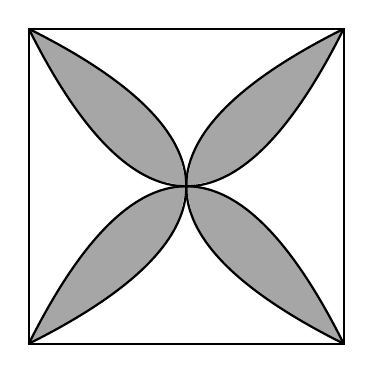
\begin{tikzpicture}[scale=1]
	
	\draw[thick] (-2,-2) rectangle (2,2);

% 1. Cánh TRÊN - PHẢI 
\fill[gray!70] plot[domain=0:2] ({sqrt(2*\x)}, {\x}) -- plot[domain=2:0] ({\x}, {sqrt(2*\x)}) -- cycle;

% 2. Cánh TRÊN - TRÁI 
\fill[gray!70] plot[domain=0:2] ({-sqrt(2*\x)}, {\x}) -- plot[domain=-2:0] ({\x}, {sqrt(-2*\x)}) -- cycle;

% 3. Cánh DƯỚI - PHẢI 
\fill[gray!70] plot[domain=0:2] ({\x}, {-sqrt(2*\x)}) -- plot[domain=2:0] ({\x}, {-0.5*(\x)^2}) -- cycle;

% 4. Cánh DƯỚI - TRÁI (Cánh còn lại)
\fill[gray!70] plot[domain=0:-2] ({\x}, {-sqrt(-2*\x)}) -- plot[domain=-2:0] ({\x}, {-0.5*(\x)^2}) -- cycle;

		\foreach \s in {-1,1} {
			\draw[thick] plot[domain=-2:2, samples=100] ({\x}, {\s*0.5*\x*\x});
			\draw[thick] plot[domain=-2:2, samples=100] ({\s*0.5*\x*\x}, {\x});
		}
	\end{tikzpicture}
}
\shortans{$32$}
\loigiai{
\immini{
Chọn hệ tọa độ như hình vẽ (1 đơn vị trên trục bằng $10\text{cm} = 1\text{dm}$).\\
Diện tích một cánh hoa (nằm trong góc phần tư thứ nhất) bằng diện tích hình phẳng giới hạn bởi hai đồ thị hàm số $y = \dfrac{x^2}{2}$, $y = \sqrt{2x}$ và hai đường thẳng $x = 0$; $x = 2$. Khi đó,
	$$S_1 = \int_{0}^{2} \left(\sqrt{2x} - \dfrac{x^2}{2}\right) \text{d}x = \dfrac{4}{3} (\text{dm}^2).$$
Diện tích tráng men cả 4 cánh hoa là 
$$4S_1 = \dfrac{16}{3} (\text{dm}^2) = \dfrac{0,16}{3} (\text{m}^2).$$
 Do đó chi phí để phủ một lớp men 4 cánh hoa là $$600 \times \dfrac{0,16}{3} = 32 \ \ \ \text{(nghìn đồng)}.$$ }
{
	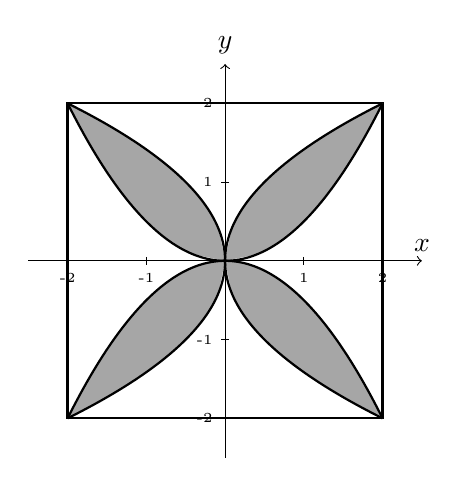
\begin{tikzpicture}[scale=1]
	\draw[->] (-2.5,0)--(2.5,0) node[above]{$x$};
	\draw[->] (0,-2.5)--(0,2.5) node[above]{$y$};
	
	% --- Thay thế cho phần vẽ vạch và điền số Ox cũ ---
	\foreach \x in {-2, -1, 1, 2} {
		\draw (\x, 0.05) -- (\x, -0.05); % Vẽ vạch chia
		\node[below, yshift=-1pt] at (\x, 0) {\tiny \x}; % Điền số tự động theo biến \x
	}
	
	% --- Thay thế cho phần vẽ vạch và điền số Oy cũ ---
	\foreach \y in {-2, -1, 1, 2} {
		\draw (0.05, \y) -- (-0.05, \y); % Vẽ vạch chia
		\node[left, xshift=-1pt] at (0, \y) {\tiny \y}; % Điền số tự động theo biến \y
	}
	
	\draw[thick] (-2,-2) rectangle (2,2);
	
	% 1. Cánh TRÊN - PHẢI 
	\fill[gray!70] plot[domain=0:2] ({sqrt(2*\x)}, {\x}) -- plot[domain=2:0] ({\x}, {sqrt(2*\x)}) -- cycle;
	
	% 2. Cánh TRÊN - TRÁI 
	\fill[gray!70] plot[domain=0:2] ({-sqrt(2*\x)}, {\x}) -- plot[domain=-2:0] ({\x}, {sqrt(-2*\x)}) -- cycle;
	
	% 3. Cánh DƯỚI - PHẢI 
	\fill[gray!70] plot[domain=0:2] ({\x}, {-sqrt(2*\x)}) -- plot[domain=2:0] ({\x}, {-0.5*(\x)^2}) -- cycle;
	
	% 4. Cánh DƯỚI - TRÁI (Cánh còn lại)
	\fill[gray!70] plot[domain=0:-2] ({\x}, {-sqrt(-2*\x)}) -- plot[domain=-2:0] ({\x}, {-0.5*(\x)^2}) -- cycle;
	
	\foreach \s in {-1,1} {
		\draw[thick] plot[domain=-2:2, samples=100] ({\x}, {\s*0.5*\x*\x});
		\draw[thick] plot[domain=-2:2, samples=100] ({\s*0.5*\x*\x}, {\x});
	}
\end{tikzpicture}
}
}
\end{ex}

\begin{ex}%[Đề khảo sát TN THPT 2025 môn Toán lần 2 trường chuyên Hà Nội – Amsterdam] %[Anh Lan Dương, 32-25-12-HaNoi-Amsterdam-L2]%[2D1C3-6]
	\immini{
	Một nhóm bạn đang thiết kế một chiếc lều cắm trại có dạng hình chóp tứ giác đều. Để đáp ứng nhu cầu sử dụng, nhóm bạn yêu cầu chiếc lều có thể tích là $8\text{ m}^3$ . Biết rằng phần vải bạt chỉ dùng để làm 4 mặt bên của lều, hãy xác định độ dài cạnh bên của chiếc lều sao cho lượng vải bạt cần dùng là ít nhất có thể. (Làm tròn kết quả đến hàng phần trăm)}
{
	\begin{tikzpicture}[line join=round, line cap=round, scale=1.5]
		\clip (-0.3, -1.1) rectangle (4,3);
		\path
		(0,0) coordinate (A) 
		(2.5,0.5) coordinate (D)
		(1.5,-1) coordinate (B) 
		($(B)+(D)-(A)$) coordinate (C)
		(0,3) coordinate (A')
		($(B)+(0,3)$) coordinate (B')
		($(C)+(0,3)$) coordinate (C')
		($(D)+(0,3)$) coordinate (D')
		(A) -- (C) coordinate[pos=0.5] (O)
		($(O)+(0,3)$) coordinate (S)
		($(A)!0.65!(B)+(35:0.65)$) coordinate (N)
		;
		% Vẽ các cạnh khuất (nét đứt)
		\draw[dashed] (S) -- (D)	(A) -- (D)-- (C); 
		
		% Vẽ các mặt và cạnh nhìn thấy (nét liền)
			\draw[thick] (S) -- (A)		(S) -- (B) 		(S)--(C) 	(B) -- (C)  
				(A)--($(A)!0.25!(B)$)--++(60:1) coordinate (M) -- ($(A)!0.65!(B)$) --(B)
				(M)..controls +(-80:0.5) and +(160:0.5) ..(N)
				(N)..controls +(-160:0.5) and +(30:0.5) ..($(A)!0.65!(B)$)
		;
	\end{tikzpicture}
}
\shortans{$3{,}24$}
\loigiai{
\begin{center}
		\begin{tikzpicture}[line join=round, line cap=round, scale=1.5]
		\path
		(0,0) coordinate (A) 
		(3,0) coordinate (D)
		(-1.,-1.) coordinate (B) 
		($(B)+(D)-(A)$) coordinate (C)
		(0,3) coordinate (A')
		($(B)+(0,3)$) coordinate (B')
		($(C)+(0,3)$) coordinate (C')
		($(D)+(0,3)$) coordinate (D')
		(A) -- (C) coordinate[pos=0.5] (O)
		($(O)+(0,3)$) coordinate (S)
		($(C)!0.5!(D)$) coordinate (I)
		;
		% Vẽ các cạnh khuất (nét đứt)
		\draw[dashed] (B)--(A)--(S)		(A)--(D)		(A)--(C)	(B)--(D)
		(S)--(O)--(I)
		;
		% Vẽ các mặt và cạnh nhìn thấy (nét liền)
		\draw[thick]	(S) -- (B) 	(S)--(D)	(S)--(C) 	(B) -- (C)--(D)  
		(S)--(I)
		;
		% Đánh dấu điểm
		\foreach \p/\pos in {A/left, B/left, C/right, D/right, S/above, O/below,
		I/below right}
		\filldraw[] (\p) circle (1.pt) node[\pos, black] {\p};
	\end{tikzpicture}
\end{center}
Gọi độ dài cạnh đáy là $x$ ( đơn vị mét, $x > 0$). Khi đó, 
$S_{\text{đáy}} = x^2$.\\
Theo đề bài, ta có:
\allowdisplaybreaks
$\begin{aligned}[t]
	8 &= \dfrac{1}{3} \cdot SO \cdot x^2  \Rightarrow SO = \dfrac{24}{x^2}; \\
	SI &= \sqrt{SO^2 + OI^2} = \sqrt{\dfrac{576}{x^4} + \dfrac{x^2}{4}};\\
	S_{\text{bạt}} &= 4S_{\Delta SCD} 
	= 4\cdot \dfrac{1}{2}\cdot CD \cdot SI 
	= 2x \sqrt{\dfrac{576}{x^4} + \dfrac{x^2}{4}} = \sqrt{\dfrac{2304}{x^2} + x^4}.
\end{aligned}$\\
mà $\dfrac{2304}{x^2} + x^4 = \dfrac{1152}{x^2} + \dfrac{1152}{x^2} + x^4 \ge 3\sqrt[3]{1152 \cdot 1152}$. Suy ra:
$S_{\text{bạt}} \ge \sqrt{3\sqrt[3]{1152^2}} \approx 18,18\text{m}^3$.\\
Dấu “=” xảy ra khi $\dfrac{1152}{x^2} = x^4 \Rightarrow x^6 = 1152 \Rightarrow x = \sqrt[6]{1152} \ (\approx 3,24\text{m})$.\\
Do đó, cạnh bên $SD = \sqrt{SI^2 + ID^2} = \sqrt{\dfrac{576}{x^4} + \dfrac{1}{2}x^2} = \sqrt{\dfrac{576}{\sqrt[3]{1152^2}} + \dfrac{1}{2}\sqrt[3]{1152^2}} \approx 3,24\text{m}$.\\
\textit{Nhận xét: Khi lượng vải bạt cần dùng ít nhất thì cạnh bên và cạnh đáy của chóp tứ giác đều bằng nhau!}
}
\end{ex}
\Closesolutionfile{ans}
%\indapan{6}{ans/ans-32-25-12-HaNoi-Amsterdam-L2-LC}

